% Clean CV/Resume Template, by Bennet B <dev@bennet.cc>
% CC0, Public-Domain
%
% Permission is hereby granted, free of charge, to any person obtaining a copy
% of this template and associated files (the "Template"), to deal
% in the Template without restriction, including without limitation the rights
% to use, copy, modify, merge, publish, distribute, sublicense, and/or sell
% copies of the Template, and to permit persons to whom the Template is
% furnished to do so, subject to the following conditions:
%
% The above copyright notice and this permission notice shall be included in all
% copies or substantial portions of the Template.
%
% THE TEMPLATE IS PROVIDED "AS IS", WITHOUT WARRANTY OF ANY KIND, EXPRESS OR
% IMPLIED, INCLUDING BUT NOT LIMITED TO THE WARRANTIES OF MERCHANTABILITY,
% FITNESS FOR A PARTICULAR PURPOSE AND NONINFRINGEMENT. IN NO EVENT SHALL THE
% AUTHORS OR COPYRIGHT HOLDERS BE LIABLE FOR ANY CLAIM, DAMAGES OR OTHER
% LIABILITY, WHETHER IN AN ACTION OF CONTRACT, TORT OR OTHERWISE, ARISING FROM,
% OUT OF OR IN CONNECTION WITH THE TEMPLATE OR THE USE OR OTHER DEALINGS IN THE
% TEMPLATE.
%
% based on Modern CV by Habib Semouma
% https://www.overleaf.com/latex/templates/modern-cv-slash-resume-template/vjrqdkpjckwj
%
%
\documentclass[UTF8]{article}
\usepackage{wallpaper}
\usepackage[UTF8,fontset=none]{ctex}
\usepackage{xeCJK}
\setCJKmainfont{PingFang SC}
\setCJKsansfont{PingFang SC}
\setmainfont{PingFang SC}
\setsansfont{PingFang SC}
\usepackage{geometry}
\usepackage{enumitem}
\usepackage{tikz}
\usepackage[
    unicode=true,
    bookmarks=true,
    bookmarksnumbered=false,
    bookmarksopen=true,
    bookmarksopenlevel=1,
    breaklinks=false,
    pdfborder={0 0 0},
    backref=false,
    colorlinks=false
    ]{hyperref}
\usepackage{lastpage}
\usepackage{hyphenat}
\usepackage{hyphsubst}
\usepackage{tabularx}
\usepackage{moresize}
\usepackage[document]{ragged2e}
% \usepackage{parskip}

\usepackage[scaled]{helvet}
\usepackage{fontawesome5}
\usepackage[defaultfam,tabular,oldstyle]{montserrat}
\usepackage[T1]{fontenc}
\renewcommand*\oldstylenums[1]{{\fontfamily{Montserrat-TOsF}\selectfont #1}}

\usepackage{titlesec}
\usepackage{xcolor}
\usepackage{tikz}
\usepackage{pgfornament}
\setlength{\parindent}{0pt}
\titleformat{\section}{\normalfont}{}{0pt}{}

\renewcommand{\arraystretch}{1.4}

\setlength\fboxrule{0pt}
\setlength\fboxsep{12pt}
% \setlength{\parskip}{.5\baselineskip plus 2pt}
% \renewcommand{\baselinestretch}{1.1}

\titlespacing{\section}{0pt}{1.5ex plus .1ex minus .2ex}{1pc}
%%%%%%%%%%%%%%%%%
% New Command
\newcommand{\starrating}[1]{%
    \makebox[2cm][l]{\raisebox{-0.5ex}{\foreach \x in {1,...,#1}{\textcolor{yellow}{\faStar}\hspace{0.2em}}}}
}

% 定义更大的bullet点
\renewcommand{\labelitemi}{\large$\bullet$}

%%%%%%%%%%%%%%%%%%%
\newcolumntype{Y}{>{\RaggedRight\arraybackslash}X}

% Change PDF Meta Info here
\hypersetup{
    pdftitle={郑鑫裕 - CV - 中文},
    pdfauthor={郑鑫裕},
    pdfsubject={CV}
}

% Paper size
\geometry{
    a4paper,
    left=0pt,
    right=0pt,
    top=0pt,
    bottom=0pt,
    nohead,
    % includefoot,
    nomarginpar
}

% Background Color of the Sidebar Column
% \definecolor{sidebg}{cmyk}{1, 0.02, 0, 0.56}
\definecolor{sidebg}{cmyk}{0.2, 0.05, 0.15, 0}
% \definecolor{sidebg}{rgb}{0.8, 0.8, 0.9}
% Background Color of the Main Column
\definecolor{mainbg}{cmyk}{0, 0, 0.07, 0.04}

% Text Color of the Main Column
\definecolor{maintext}{cmyk}{1, 0.02, 0, 0.8}
% Text Color of the Sidebar Column
% \definecolor{sidetext}{cmyk}{0, 0, 0.07, 0.04}
\definecolor{sidetext}{cmyk}{1, 0.02, 0.5, 0.8}
\pagecolor{mainbg}

\begin{document}
\setlength{\topskip}{0pt}\setlength{\footskip}{0pt}%
\fcolorbox{red}{sidebg}{%
    \begin{minipage}[t][\textheight-2\fboxsep-2\fboxrule][t]{\dimexpr0.40\textwidth-2\fboxrule-2\fboxsep\relax}
        \color{sidetext}
        %%%%%%%%%%%%%%%%%%%%%%%%%%%%%%%%%%%%%%%%%%%%%%%%%%%%
        % YOUR NAME, PRONOUNS, OCCUPATION(s), AND HEADSHOT
        {\bfseries\HUGE 郑鑫裕} \\
        \begin{center}
            \begin{tikzpicture}
            \clip (0,0) circle (2.5cm) node[anchor=center] at (-0.05, -0.6){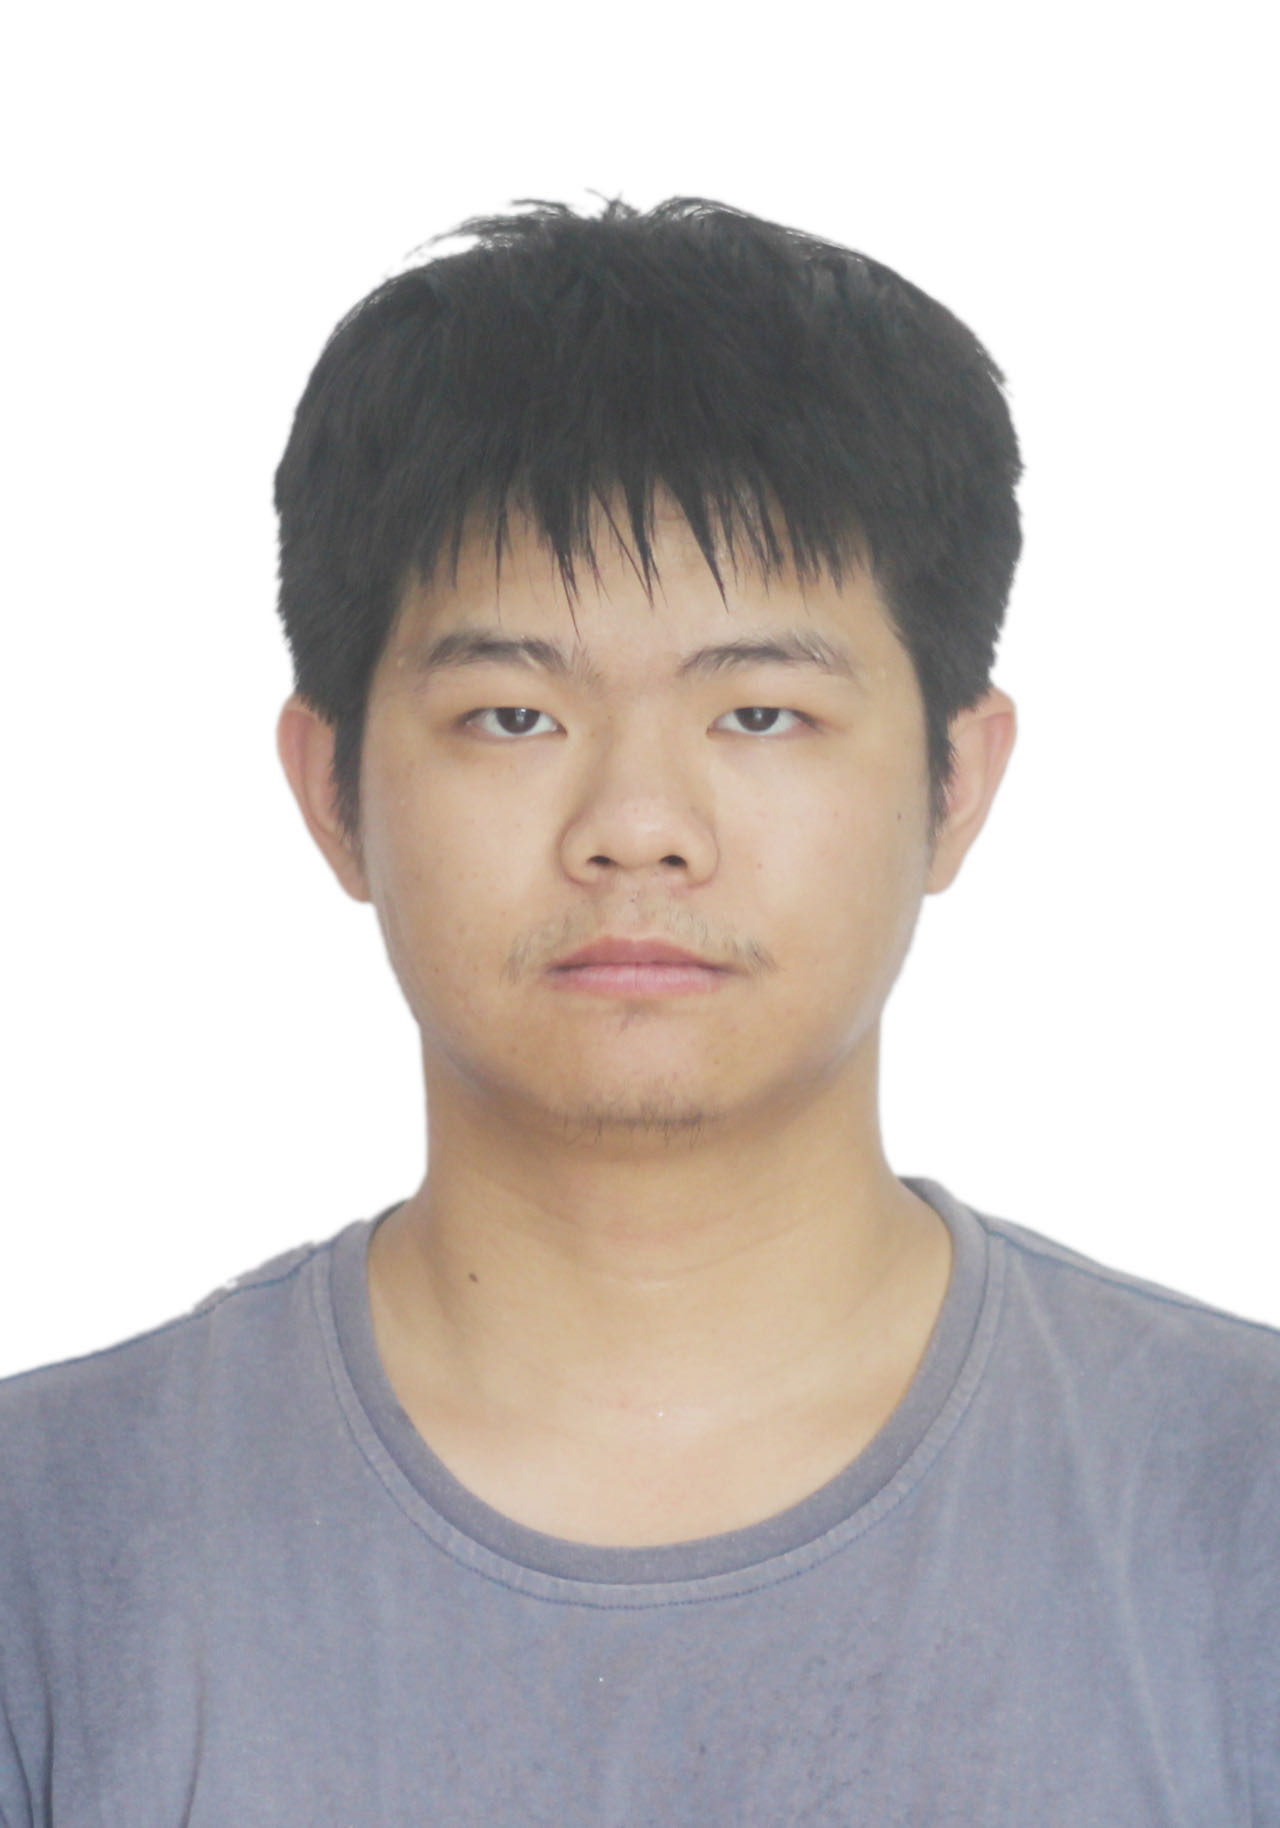
\includegraphics[width=5.2cm]{cv_picture.jpg}};
            \end{tikzpicture}
        \end{center}
        \vspace{-2.5cm}
        \rule{\linewidth}{0.4pt} \\
        %%%%%%%%%%%%%%%%%%%%%%%%%%%%%%%%%%%%%%%%%%%%%%%%%%%%
        % YOUR PERSONAL INFROMATION
        \phantomsection{}
        \addcontentsline{toc}{section}{个人信息}
        \section*{\large 个人信息}
        \begin{tabularx}{\textwidth}{cY}
            \faStarOfLife{} & 2003.11.26 \\
            \faPhone{}      & 150 7938 0535 \\
            \faEnvelope{}   & \href{mailto:3193603347@qq.com}{3193603347@qq.com} \\
            \faMapMarker{}  & 陕西省西安市西咸新区西安交通大学创新港校区惠园 \\
        \end{tabularx}
        \vspace{1pt} \\
        \rule{\linewidth}{0.4pt} \\
        \section*{\large 求职意向}
        寻求2026年4月起的实习机会，希望从事人工智能算法相关技术工作
        \vspace{1pt} \\
        \rule{\linewidth}{0.4pt}
        \section*{\large 技能}
        \vspace{-0.5cm}
        \begin{tabularx}{\textwidth}{cY}
            \faCode{}        & Python, C/C++\\
            \faPen*{}        & \LaTeX, HTML, CSS\\
            \faCode{}        & Vibe Coding\\
            \faCogs{}        & ComfyUI\\
            \faLanguage{}    & 英语：CET6 \\
            \faLanguage{}    & 法语：DELF B2 \\
        \end{tabularx}
        \vspace{1pt} \\
        \rule{\linewidth}{0.4pt}
        \section*{\large 自我评价}
        踏实肯干，学习能力强，适应能力强。具备良好的沟通协调能力。拥有国际化教育背景和跨文化视野，思维开阔。希望能加入一个有野心、有冲劲的团队，提高自己的专业能力。
    \end{minipage}
}
\hfill
\fcolorbox{red}{mainbg}{%
    \begin{minipage}[t][\dimexpr\textheight-2\fboxrule-2\fboxsep\relax][t]{\dimexpr0.6\textwidth-2\fboxrule-2\fboxsep\relax}
        \color{maintext}

\addcontentsline{toc}{section}{教育背景}
\section*{\bfseries\Large 教育背景 \rule{\linewidth}{0.4pt}}
\vspace{-0.2cm}
\begin{tabularx}{\linewidth}{X r}
    \large \textbf{ 西安交通大学} & Sept. 2025 -- Now \\
\end{tabularx}
\begin{itemize}[leftmargin=1.5em, itemsep=0.1em]
    \item 获一等学业奖学金免试升学攻读本校人工智能研究生，目前主要基于扩散模型进行图像压缩方向的研究
\end{itemize}

\begin{tabularx}{\linewidth}{X r}
    \large \textbf{ 西安交通大学} & Sept. 2021 -- July 2025 \\
\end{tabularx}
\begin{itemize}[leftmargin=1.5em, itemsep=0.1em]
    \item 人工智能专业，获中外联合培养机会，赴法完成大三大四学业
\end{itemize}

\begin{tabularx}{\linewidth}{X r}
    \large \textbf{ 法国里尔中央理工学院（双学位）} & Sept. 2023 -- July 2025 \\
\end{tabularx}
\begin{itemize}[leftmargin=1.5em, itemsep=0.1em]
    \item 通用工程师专业，CSC奖学金，在校期间担任国际学生联合会主席及中国学生联合会会计
\end{itemize}

\addcontentsline{toc}{section}{专业经历}
\section*{\bfseries\Large 专业经历 \rule{\linewidth}{0.4pt}}
\vspace{-0.2cm}

\begin{tabularx}{\linewidth}{X r}
    \large \textbf{南京炙石科技有限公司 算法实习生} & Nov. 2025 -- Feb. 2026 \\
\end{tabularx}
{视频生成算法优化：基于 Wan2.2 (Video-DiT) 训练定制化 LoRA，通过清洗企业闭源数据与优化训练策略，解决视频生成中的时序闪烁问题，显著提升模型稳定性。

视频换装工作流开发：基于 ComfyUI 搭建端到端视频换装 Pipeline，通过实现高保真细节还原，业务表现优于市面上同类方案。

图像换装：基于开源的CatVTON模型进行改进，使用本地数据进行训练，得到可用于生产的图像换装模型。

提示词工程：使用 Nano Banana 与 ChatGPT 研发用于复杂材质衣物镂空图生成的提示词，将生成成功率提升至 99\% 以上。} \\[0.6em]

\begin{tabularx}{\linewidth}{X r}
    \large \textbf{Groupe Bouygues 实习（法国）} &  May 2024 -- Aug. 2024 \\
\end{tabularx}

{开发基于AI视频理解的工地智能安全头盔系统。通过实地调研工地安全风险，识别8类主要风险场景。采用YOLOv5s-pose提取人体关键点，通过划分帧组并结合Transformer架构充分利用帧间时序信息。

在企业数据集上训练模型，最终mAP@0.5达到0.94的优异性能。基于Arduino和ESP32-CAM平台实现硬件原型，成功集成边缘计算模块，为工地安全监控提供了智能化解决方案。} \\[0.6em]

\begin{tabularx}{\linewidth}{X r}
    \large \textbf{LamCube 实习（法国）} &  Feb. 2024 -- Mar. 2024 \\
\end{tabularx}
{基于深度学习构建建筑裂缝智能检测系统。通过深入调研并分析50+篇建筑及工业领域AI检测相关文献。\\采用基于Deeplabv3+的语义分割技术方案，结合传统图像处理方法进行优化，在CrackForest数据集上进行训练，最终实现IoU达到0.84的高精度检测效果，为建筑结构安全评估提供了可靠的自动化检测工具。} \\[0.6em]

\addcontentsline{toc}{section}{荣誉与活动}
\section*{\bfseries\Large 荣誉与活动 \rule{\linewidth}{0.4pt}}
\vspace{-0.2cm}
\begin{tabularx}{\linewidth}{X r}
    \large \textbf{ CSC 奖学金} &  2023 - 2025 \\
\end{tabularx}
{由中国留学基金委授予，支持在法国里尔中央理工学院的双学位学习} \\[0.6em]

\begin{tabularx}{\linewidth}{X r}
    \large \textbf{里尔中央理工学院国际学生联合会主席} &  2024 - 2025 \\
\end{tabularx}
{协助国际学生办理入学手续，组织文化交流活动促进国际学生交流} \\[0.6em]

\begin{tabularx}{\linewidth}{X r}
    \large \textbf{里尔中央理工学院中国学生联合会会计} &  2024 - 2025 \\
\end{tabularx}
{管理学生联合会财务，组织中国传统节日庆祝活动推广中华文化} \\[0.6em]

        \vfill%
        \vfill%
    \end{minipage}
}%
\end{document}
